\begin{frame}{대전 도시철도 2호선 (32408)}

\small

\textbf{문제}

대전시는 
$N$개의 교차로와 
$N-1$개의 도로가 교차로를 정점, 도로를 간선으로 하는 트리 구조를 이루고 있다. 교차로는 
$1$번부터 
$N$번까지 번호가 매겨져 있다. 대전시는 
$1$번 교차로와 
$N$번 교차로를 잇는 경로를 따라 대전 도시철도 1호선을 운행하고 있다. 이 경로에 포함되는 교차로와 도로에는 각각 역과 철도가 설치되어 있다.

대전시는 도시철도 2호선을 추가로 운행하려고 한다. 1호선과 비슷하게 2호선도 
$S$번 교차로와 
$E$번 교차로를 잇는 경로를 따라 역과 철도를 설치하려고 한다. 
$S$번과 
$E$번 교차로는 1호선 역이 설치되지 않은 서로 다른 교차로여야 하고, 이용객이 1호선으로 환승할 수 있도록 2호선은 1호선 역을 적어도 하나 포함해야 한다.

대전 도시철도 2호선을 운행하기 위해 조건을 만족하는 두 교차로를 고르는 경우의 수를 구해보자. 단, 두 교차로의 순서를 바꾼 것은 같은 경우로 본다.

\end{frame}

\begin{frame}{예제 입력}

\centering

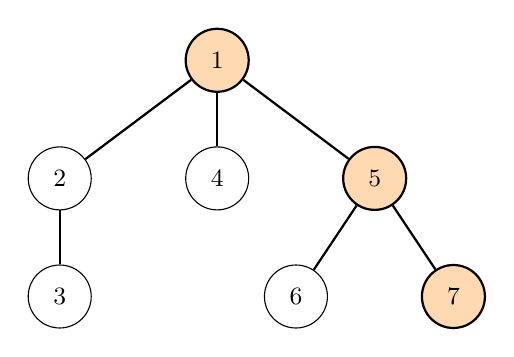
\begin{tikzpicture}[
    vertex/.style={
        circle,
        draw,
        minimum size=8mm,
        font=\small
    },
    highlight/.style={
        circle,
        draw,
        fill=orange!30,
        thick,
        minimum size=8mm,
        font=\small
    },
    edge/.style={
        thick
    },
    every node/.style={vertex}
]

% Nodes
\node[highlight] (1) at (0,0) {1};

\node (2) at (-2,-1.5) {2};
\node (3) at (-2,-3) {3};

\node (4) at (0,-1.5) {4};

\node[highlight] (5) at (2,-1.5) {5};
\node (6) at (1,-3) {6};
\node[highlight] (7) at (3,-3) {7};

% Edges
\draw[edge] (1) -- (2);
\draw[edge] (2) -- (3);

\draw[edge] (1) -- (4);

\draw[edge] (1) -- (5);
\draw[edge] (5) -- (6);
\draw[edge] (5) -- (7);

\end{tikzpicture}

\end{frame}

\setproblem{32408}

\begin{frame}[fragile, allowframebreaks]{정의찬 소스 코드}
\inputminted{java}{\prob/Uichan.java}
\end{frame}

\begin{frame}[fragile, allowframebreaks]{원찬혁 소스 코드}
\inputminted{java}{\prob/Chanhyeok.java}
\end{frame}

\begin{frame}[fragile, allowframebreaks]{손현준 소스 코드}
\inputminted{java}{\prob/Hyeonjun.java}
\end{frame}

\begin{frame}[fragile, allowframebreaks]{서민종 소스 코드}
\inputminted{java}{\prob/Minjong.java}
\end{frame}

\begin{frame}[fragile, allowframebreaks]{김준형 소스 코드}
\inputminted{java}{\prob/Junhyeong.java}
\end{frame}

\begin{frame}[fragile, allowframebreaks]{김시온 소스 코드}
\inputminted{java}{\prob/Sion.java}
\end{frame}

% \begin{frame}[fragile, allowframebreaks]{김지훈 소스 코드}
% \inputminted{java}{\prob/Jihoon.java}
% \end{frame}

\begin{frame}[fragile, allowframebreaks]{임건애 소스 코드}
\inputminted{java}{\prob/Keonae.java}
\end{frame}

